\chapter{Common Analysis Items}
\label{chapter:CommonAnalysisItems}

%todo IO muons
%todo
After collisions in the LHC, the particles hits exist as different electronic signals from various detector components saved in hard disk, converting these signals into physics objects worth analyzing takes different reconstruction, identification, cleaning, and calibration steps. This chapter will discuss the different steps these detector hits go through before they become analysis-ready physics objects. 

\begin{figure}[!htb]
    \begin{center}
        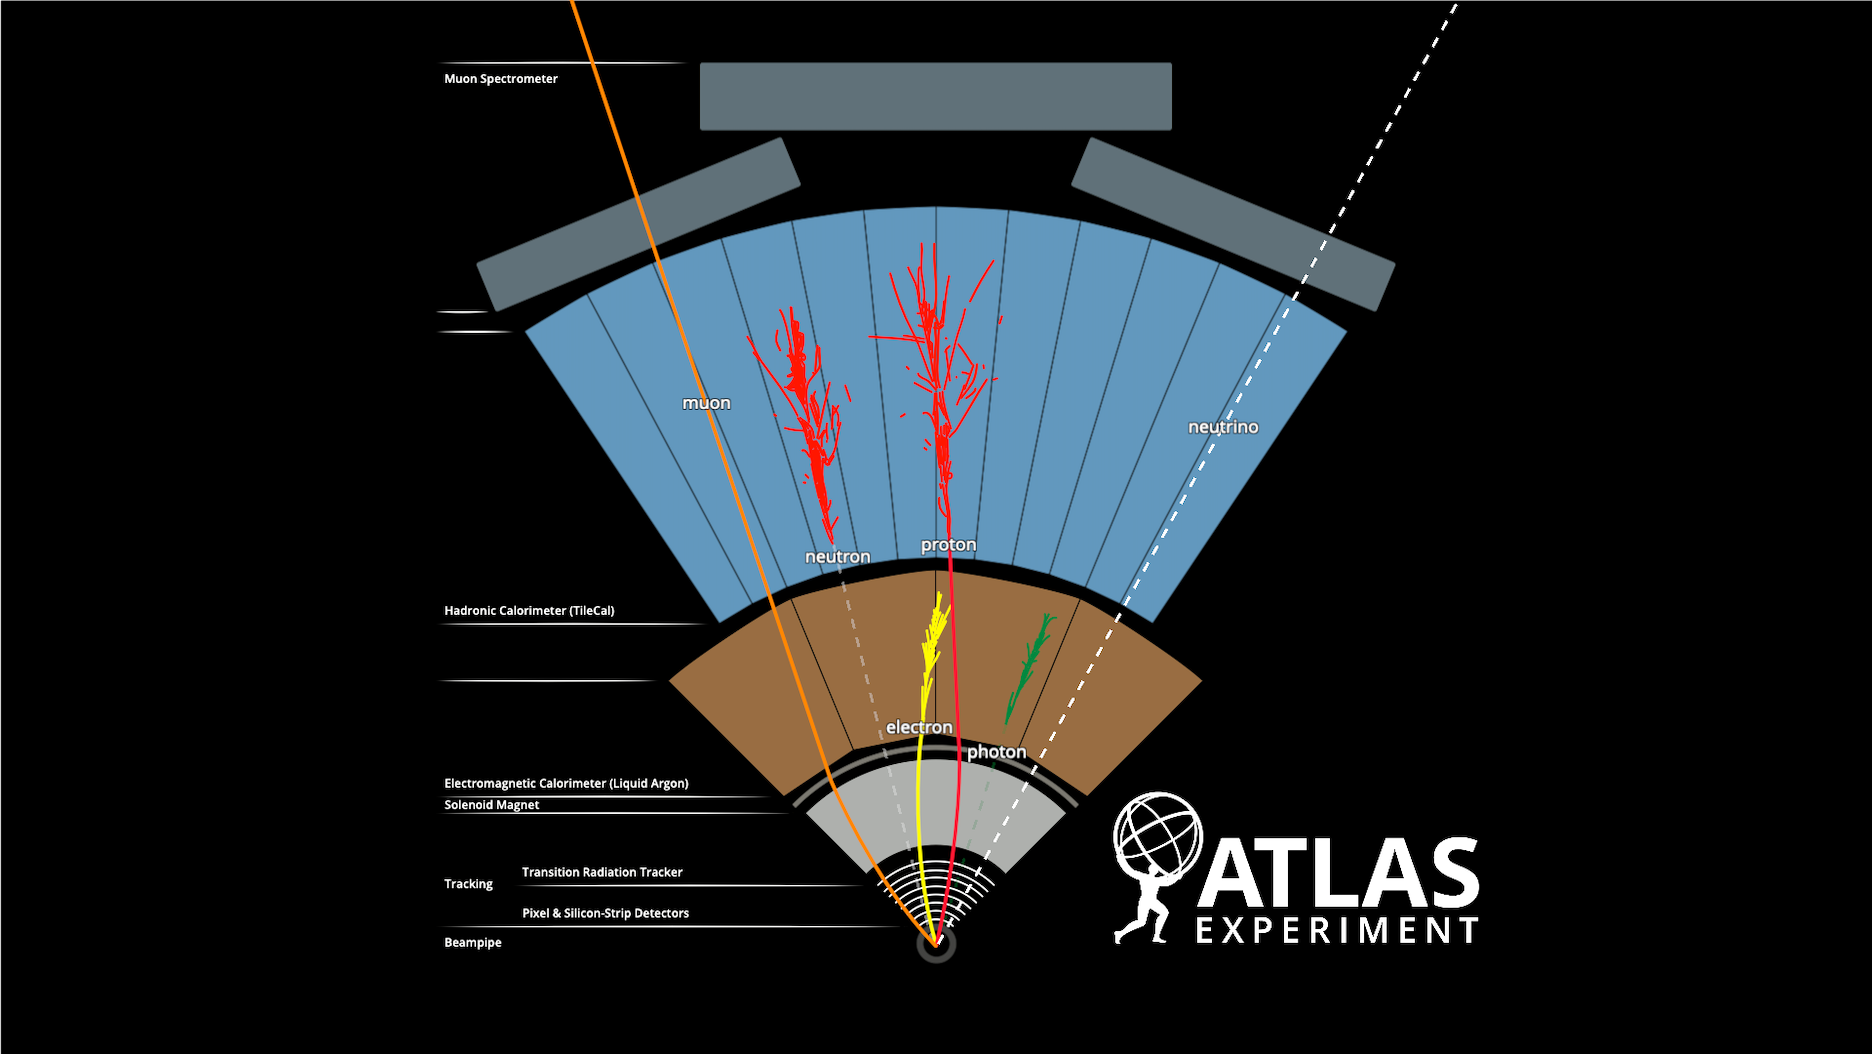
\includegraphics[width=1.1\textwidth]{figures/common_ana/ParticleSignature}
        \caption{        
            Different particles displays a different particle signature characteristics in the ATLAS detector\cite{Mehlhase:2770815}.
        }
        \label{fig:isolationWP}
    \end{center}
\end{figure}

\section{Tracks and primary vertices}

Charged particles leave trajectories in two distinct ATLAS sub-detector systems, namely the inner detector(ID) and the muon system(MS). The inner detector is made up of the pixel detector, the Semiconductor Tracker, and the Transition Radiation Tracker(TRT). Tracking is done for all particles that are charged. 
The MS is made up of Monitored Drift Tubes(MDTs), the Cathode Strip Chambers(CSC), Thin Gap Chambers(TGC), and the Resistive Plate Chambers(RPC). It's mainly used for
track formation of muons, which are minimizing particles that through all of the ID and calorimeters.


\subsection*{Tracks}
To reconstruct a hit from detector raw hit information, a couple of  coincidence measurement across the different subsystems will be used to form a track seed. Then, a Kalman filter is used to fit the tracks,  irrelevant hits from pile-up are removed through the filter rejection.  
A track formed this way is described by the following few track-associated parameters: ($d_{0}$, $z_{0}$, $\phi$, $\theta$, q/p).
%by forward filtering, backward smoothing and outlier rejection of

\begin{figure}[!htb]
    \begin{center}
        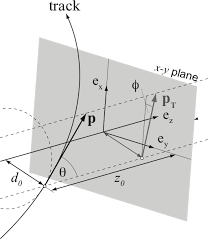
\includegraphics[width=0.45\textwidth]{figures/common_ana/Track}
        \caption{ 
            Track reconstruction in ATLAS. Schematic view of how the parameters associated with track creation.
        }
        \label{fig:isolationWP}
    \end{center}
\end{figure}


\subsection*{Primary Vertex}
Once tracks are formed in the inner detector, primary vertices can be constructed to discriminate an event from other hits. 
Primary vertices are the initial interaction point where the further decay particles that reach the ATLAS detector are formed. Verticing is important as it is effective in discriminating pile-up hits from the ones from the event-of-interest. This is increasingly important in newer LHC runs where the higher luminosity has resulted in additional in-time and out-of-time pile-ups. 

\begin{figure}[!htb]
    \begin{center}
        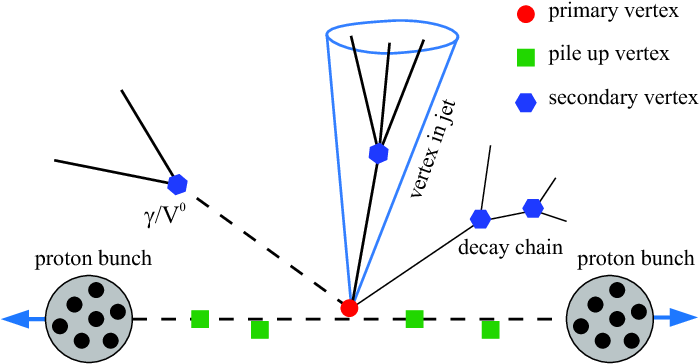
\includegraphics[width=0.75\textwidth]{figures/common_ana/Vertex}
        \caption{        
            Schematic view showing vertexing in ATLAS\cite{4774734}.
        }
    \end{center}
\end{figure}
Vertexing is consist of a couple of different steps:

1. A vertex seed is found by filtering the point where most interactions are found. This is done by an iterative method or imaging method.  

2. Tracks consistent with the chosen vertex seed are put into a group.

3. An adaptive vertex fitting algorithm is used to find the position and the associated error of the vertex. 

4. The unused tracks are used for the next vertex creation. 

There are usually a couple of primary vertices in each bunch crossing, the vertex with the highest PT particles originated from it is considered the hard-primary vertex of the event, the others are considered the pile-up primary vertices. 

With tracks and primary vertices constructed, particle reconstruction can begin. 


\section{Muons}
Muons on ATLAS formed from the tracking and primary vertex information from both the ID and the MS described in the above section. Additinoal information from the calorimeter is also used. There are four main muon reconstruction strategies. Mainly due to different PT muon in different detector location will require different strategies for optimal reconstruction efficiency. There are four muon working points, which uses different reconstruction strategy combination and discriminating cuts to
increase the identification efficiency for different analyses.

\begin{figure}[!htb]
    \begin{center}
        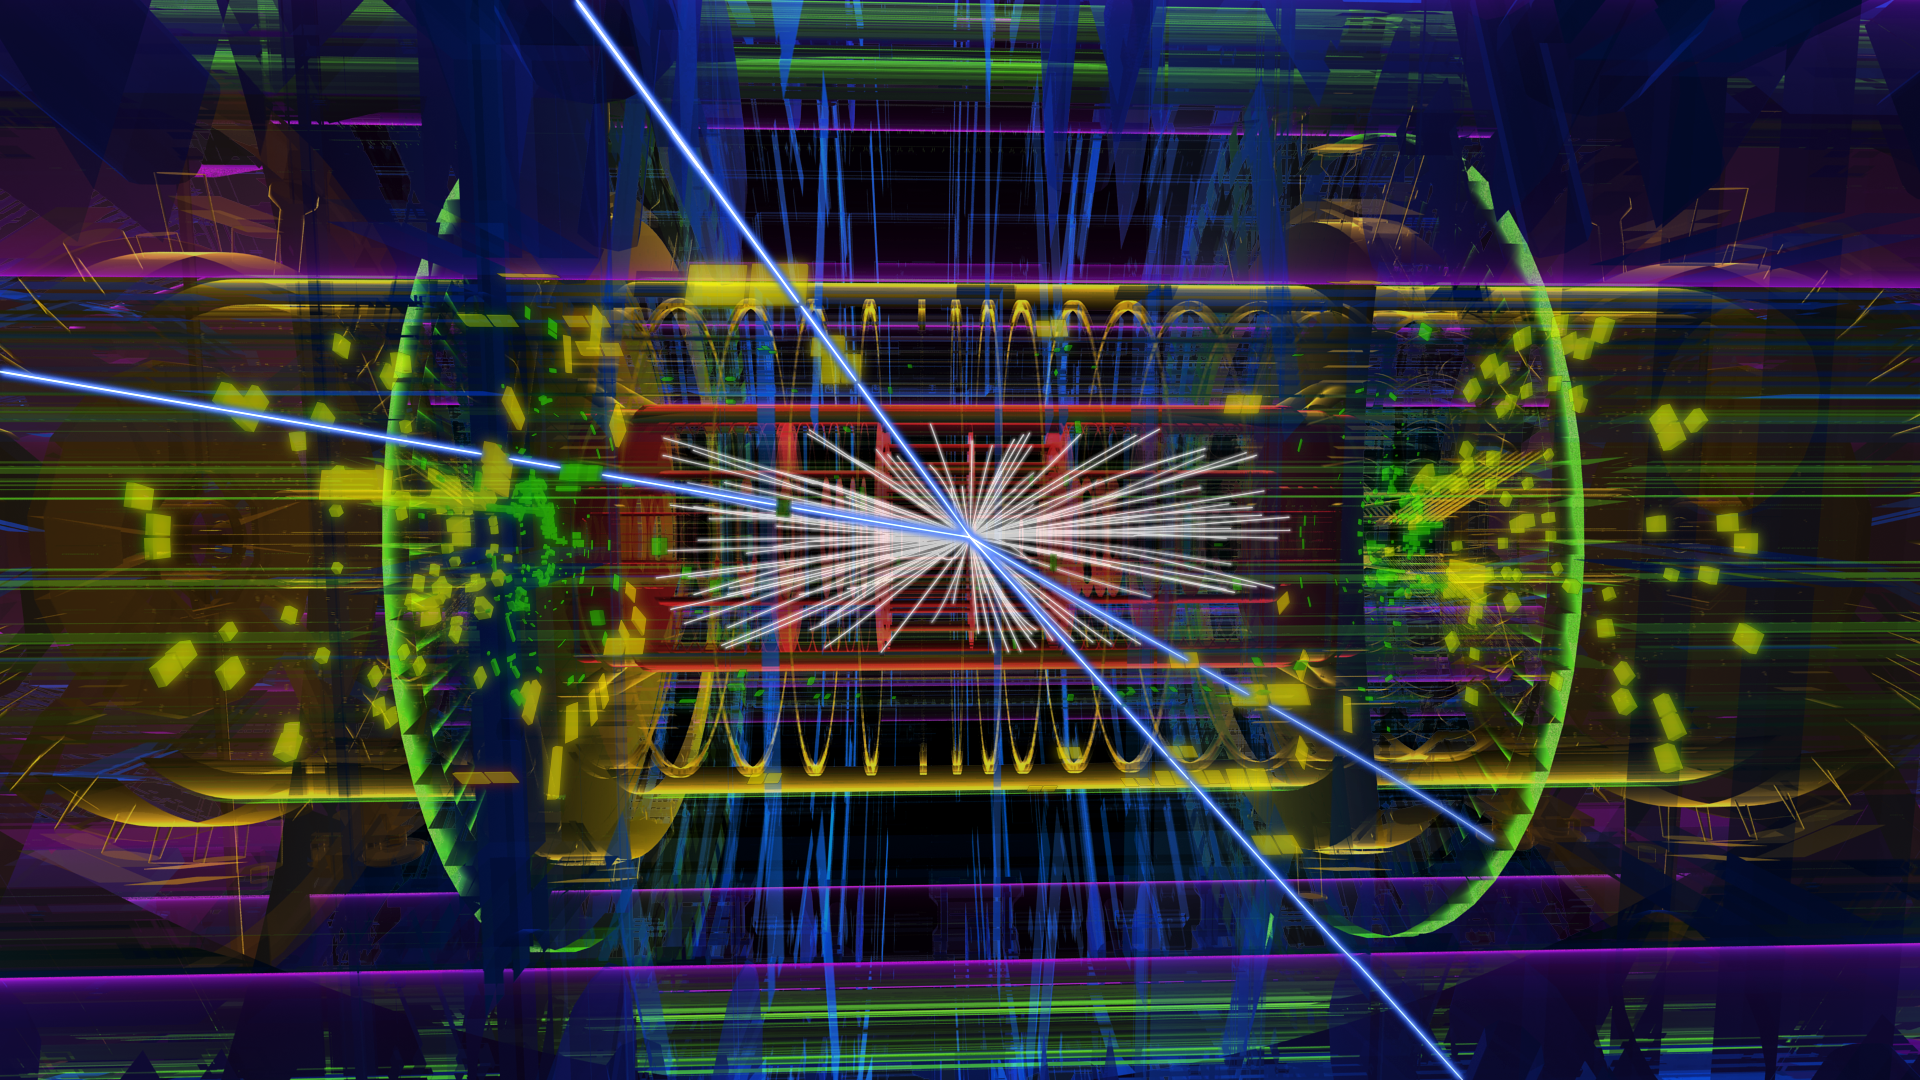
\includegraphics[width=0.85\textwidth]{figures/common_ana/Muon}
        \caption{        
            Event visualization of a four muon event in the ATLAS detector\cite{ATLAS:1697053}.
        }
    \end{center}
\end{figure}

These strategies and working points are result from studies done on the standard samples of Z to $\mu \mu $ and $J/\Psi$ to \mu \mu. 
%As different muon transverse momentum will lead to muon hits depositing in different parts of the detector and different region also require different strategy for best differentiation. 
%forward region also present more difficult muon finding conditions, given this four different muon algorithms are developed. 

\subsection{Muon Reconstruction}
A similar principle is utilized for all four strategies: tracks are found in one part of the detector through pattern finding from hit patterns in the chambers. At least two matching segments from different subdetector parts is needed to form a track candidate. From the track candidate, a couple of global $\chi^{2}$ fits is done to associate other hits and drop outlier from the fit, while removing the outlier hits. The main goal of muon reconstruction is to increase the
reconstruction efficiency, which is the ratio between muon reconstructed and the number of truth muons. 

\begin{itemize}
\item Combined (CB) muon
This strategy is optimal for the muons that are detected in both the ID and the MS in both the barrel region and end-cap region of the detector. Tracks are each constructed from the ID and the MS and a global refit done to remove outliers to improve the fit quality. This is mostly done by an outside-in approach where the tracks in MS are made to match the ones seen in the ID. 

\item Inside-out(IO) muons
    This strategy complements the Combined muon approach and finds muons from an inside-out algorithm. It looks for MS hits that can be associated with ID tracks and recovers some muons that don't make it to the MS fully. 

\item Segment-tagged (ST) muons
This method is used to identify lower PT muons that couldn't make it to multiple layer of the MS. If a track in the ID can be matched to at least one track segment in the MDT in the barrel or CSC in the end-cap, it will be selected as a segment-tagged muon. 

\item Calorimeter-tagged(CT) muon
This method is for even lower PT muons that could not make it to the MS at all. Muons between 15 < $P_{T}$ < 100GeV is formed from matching a track in ID with energy deposit in the calorimeter that matches the minimum-ionizing particle. This is optimized for barrel muons of $|\eta <0.1|$. 

\item Extrapolated(ME) muon}
This strategy is for muons that are very forward and is swamp under noise from pile-up. Muon tracks in the MS chamber with a loose compatibility to the originating IP are ME muons are accepted as ME muons. This strategy extending the acceptance of muons in the forward region from 2.5< $|\eta|$<2.7, where there is no ID coverage and cannot be reconstructed by the above other methods.

\end{itemize}

\subsection{Muon Identification}
Muon identification is a set of selection criteria done on the candidate muons to cut out background from pions/kaon decays that would form muons that are not of interest to analysis. This increases the analysis signal sensitivity. In different analyses, depending on the signal type, different muon identification working points are used.

A couple of criteria are used for muon identification: $q/p_{significance}$, $\rho'$ and $\chi^{2}_{norm}$. They are defined as below:

\subsubsection*{Discrimination Criteria}
\begin{itemize}

\item q/p significance
    \begin{equation}
    $$ q/p_{significance} = |(q/p)^{ID} - (q/p)^{MS}|/\sqrt{\sigma^{MS}_{PT} + \sigma^{ID}_{PT}} $$
    \end{equation}

This is the absolute value of the difference between the charges and the PT measurement divided by the sum of error in the PT measurement of both the ID and MS.

\item $\rho'$
    \begin{equation}
    $$ \rho' = |P_{T}^{MS} - P_{T}^{ID}| / P_{T}^{Combined} $$
    \end{equation}

This is the absolute value of the difference between the PT of the MS and the ID divided by the combined PT of the muon candidate.

\item $\chi_{norm}^{2}$

    This is the $chi^{2}$ of the fit from the combined muon track from both the ID and MS.

\end{itemize}

These selection criteria for the muon groups above result in five different working points.


\subsubsection*{Muon Working Points}
\begin{itemize}

\item MEDIUM \newline
This is the most commonly used working point. q/p significance $<$ 7. It accepts only the CB and IO muons.  

\item LOOSE \newline
    The loose working point accepts all the muons that pass the medium working point. It also accepts low-PT muons, including IO muons with PT lower than 7GeV. Some ST and CT muons are also accepted if they pass certain requirements. 

\item TIGHT \newline
    This working point accepts a subset of the medium working point muons. In addition, they are required to have a normalized $\chi^{2}$ of less than 8. The requirement on q/p compatibility and $\rho'$ depends on $\eta$ and $P_{T}$ of the muon.

\item HIGH $P_{T}$ \newline
This working point only accept muons that also pass the medium working point requirement. Owing to their high PT, the reconstruction can be done with the MS alone for a higher resolution.


\item LOW $P_{T}$ \newline
The Low-$p_{T}$ working point includes all of the muons in the medium working point, it's identical to the medium working point muon set above $P_{T}=18GeV$. But this working point also includes muons with lower pt that does not make it to the middle of the MS, this working point includes muons down to 3 GeV. 

\end{itemize}

\begin{figure}[!htb]
    \begin{center}
        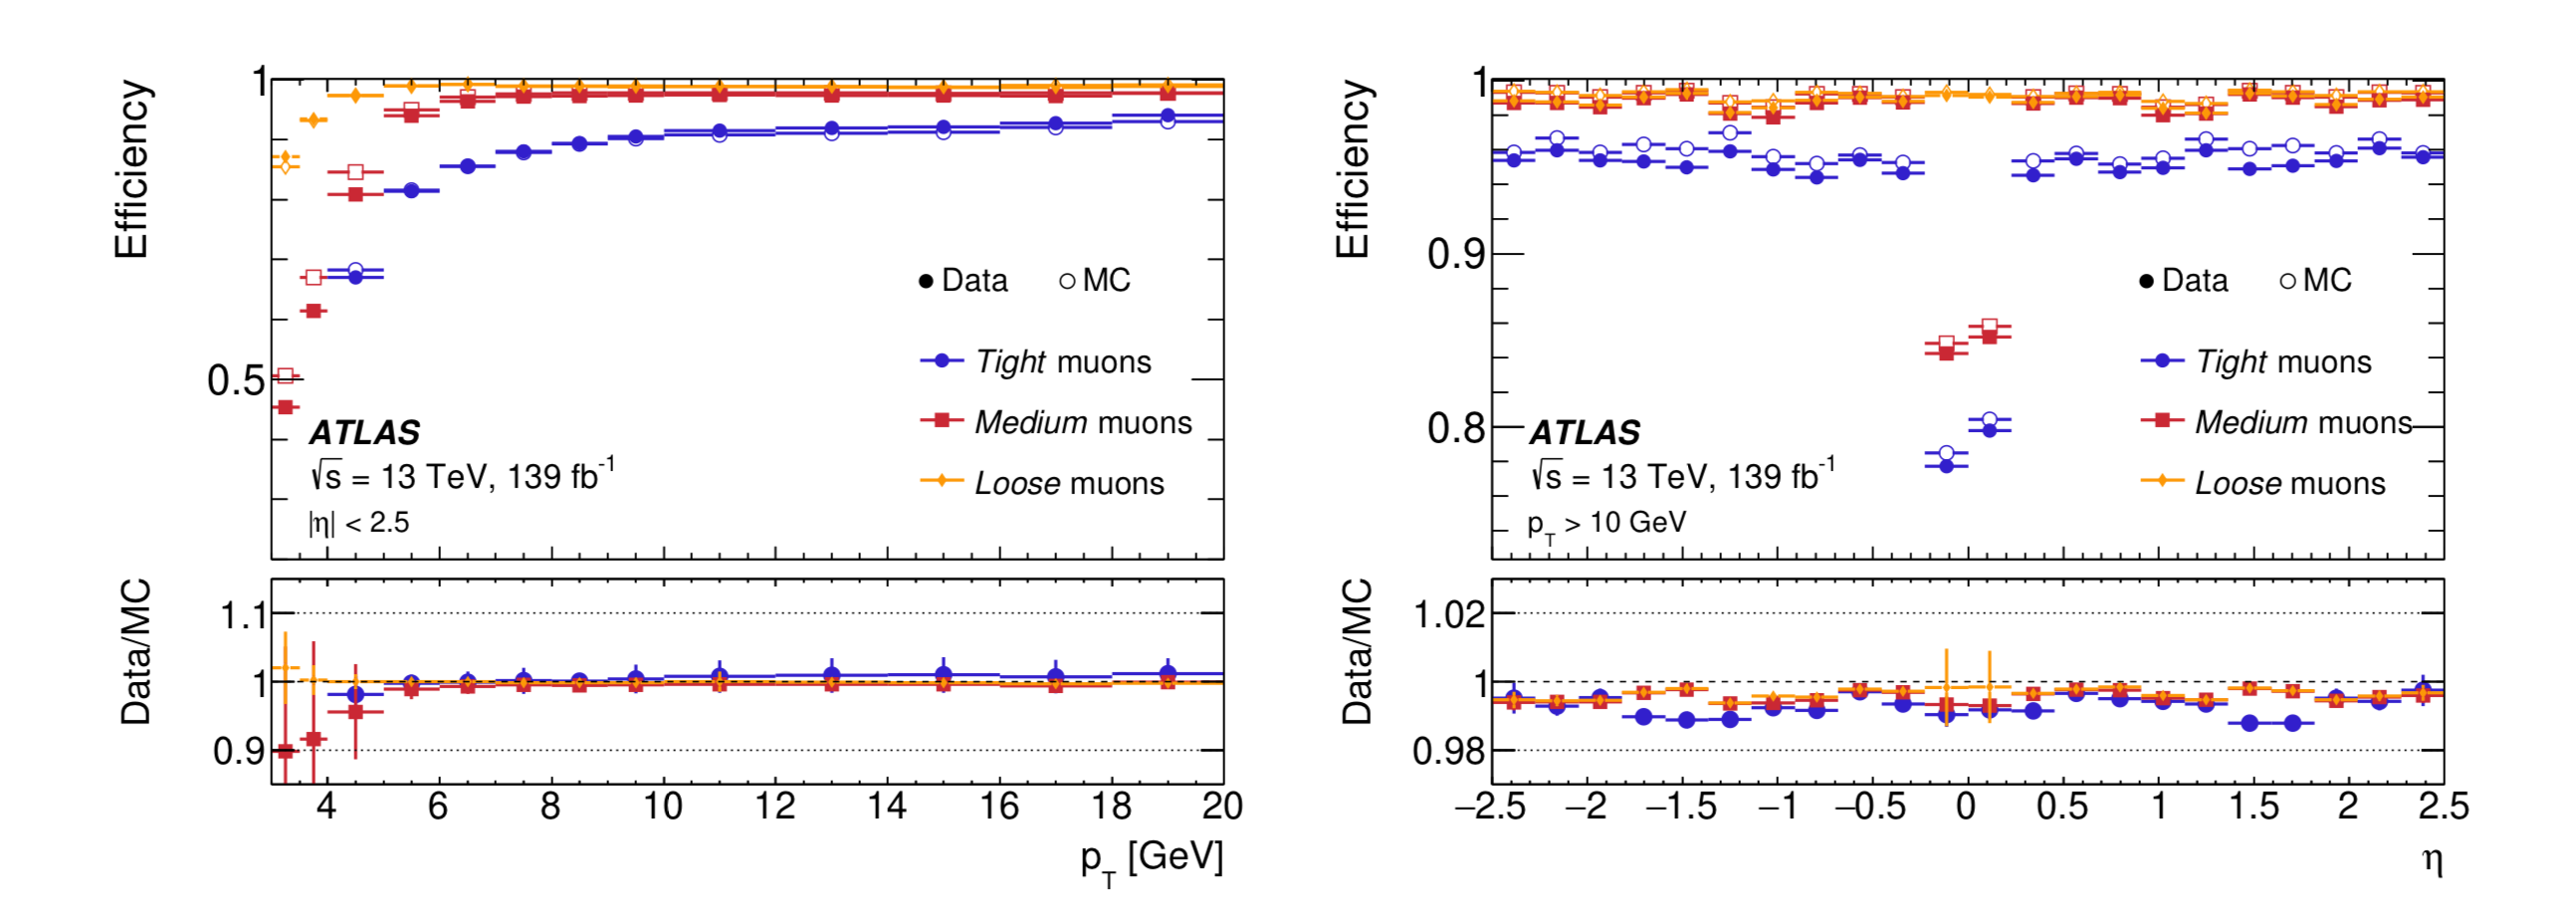
\includegraphics[width=1\textwidth]{figures/common_ana/IdentificationEff}
        \caption{
            This figure shows the reconstruction and identification efficiencies in different variable range in different working points\cite{Aad:2746302}.
    }
        \label{fig:isolationWP}
    \end{center}
\end{figure}



\subsection{Muon Isolation}
In addition to the reconstruction and identification working point, muon isolation is to pick out the muon candidates of interest and drop other ones to the analysis for better sensitivity. On ATLAS, the interesting leptons came from the hard primary vertex decay of radially decaying particles. W, Z, Higgs bosons or other BSM particles such as the Z' are examples decays that concern analyzers. Muons formed are known as "prompt muons", usually clean and do not have many associated neighboring hits. Less interested muons came from the semileptonic decay from jet fragmentation, these muons decays are formed with lots of
neighboring hits. The neighboring hits can be used as criteria to discriminate interesting muons from the less interesting ones, the step is called muon isolation. This increases the signal sensitivity by cutting down the background in searches and measurements.
%They are often classified as "background" processes. To distinguish these leptons and increase signal significance for the lepton
%from processes that concerns us, an isolation criteria is used. 
There are two variables used for muon isolation, one is track-based isolation and the other is calorimeter-based isolation. 

\subsubsection*{Isolation Parameters}
The parameters used in the isolation criteria are defined as the following:
\begin{itemize}
    \item  $P_{T}^{varcone\:size}$ \newline
        The track-based isolation variable, $P_{T}^{varcone\:size}$ are the sum of the PT of all the tracks in a variable-sized cone. The variable-sized cone(varcone) is defined as below.

    
\[ \delta R = min(\frac{10}{P^{\mu}_{T}[GeV]}, \delta R_{max}) \]
The term is PT dependent, the larger the PT, the smaller the cone. 
    \item $E^{topocone\:size}_{T}$ \newline

        A calorimeter based parameter $E^{topocone\:size}_T$ is defined as the sum of the energy deposit in a $\delta R$ size topo cone. 

\end{itemize}

The isolation criteria using the track-based variable is the isolation variable to the transverse momentum to the muon. Studies are done on data Monte Carlo to get the best cut-off point. The different working points are listed as below~\ref{fig:isolationWP}.

%\section{Muon scale and resolution}

\begin{figure}[!htb]
    \begin{center}
        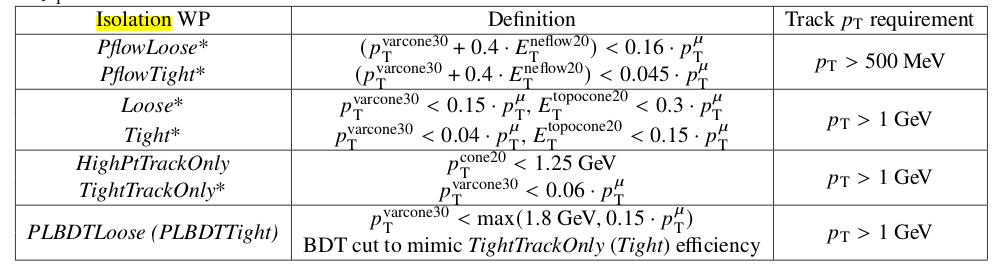
\includegraphics[width=0.75\textwidth]{figures/common_ana/Isolation}
        \caption 
        {
            This figure shows the isolation working points on ATLAS from full run2\cite{Aad:2746302}.}
        \label{fig:isolationWP}
    \end{center}
\end{figure}

\begin{figure}[!htb]
    \begin{center}
        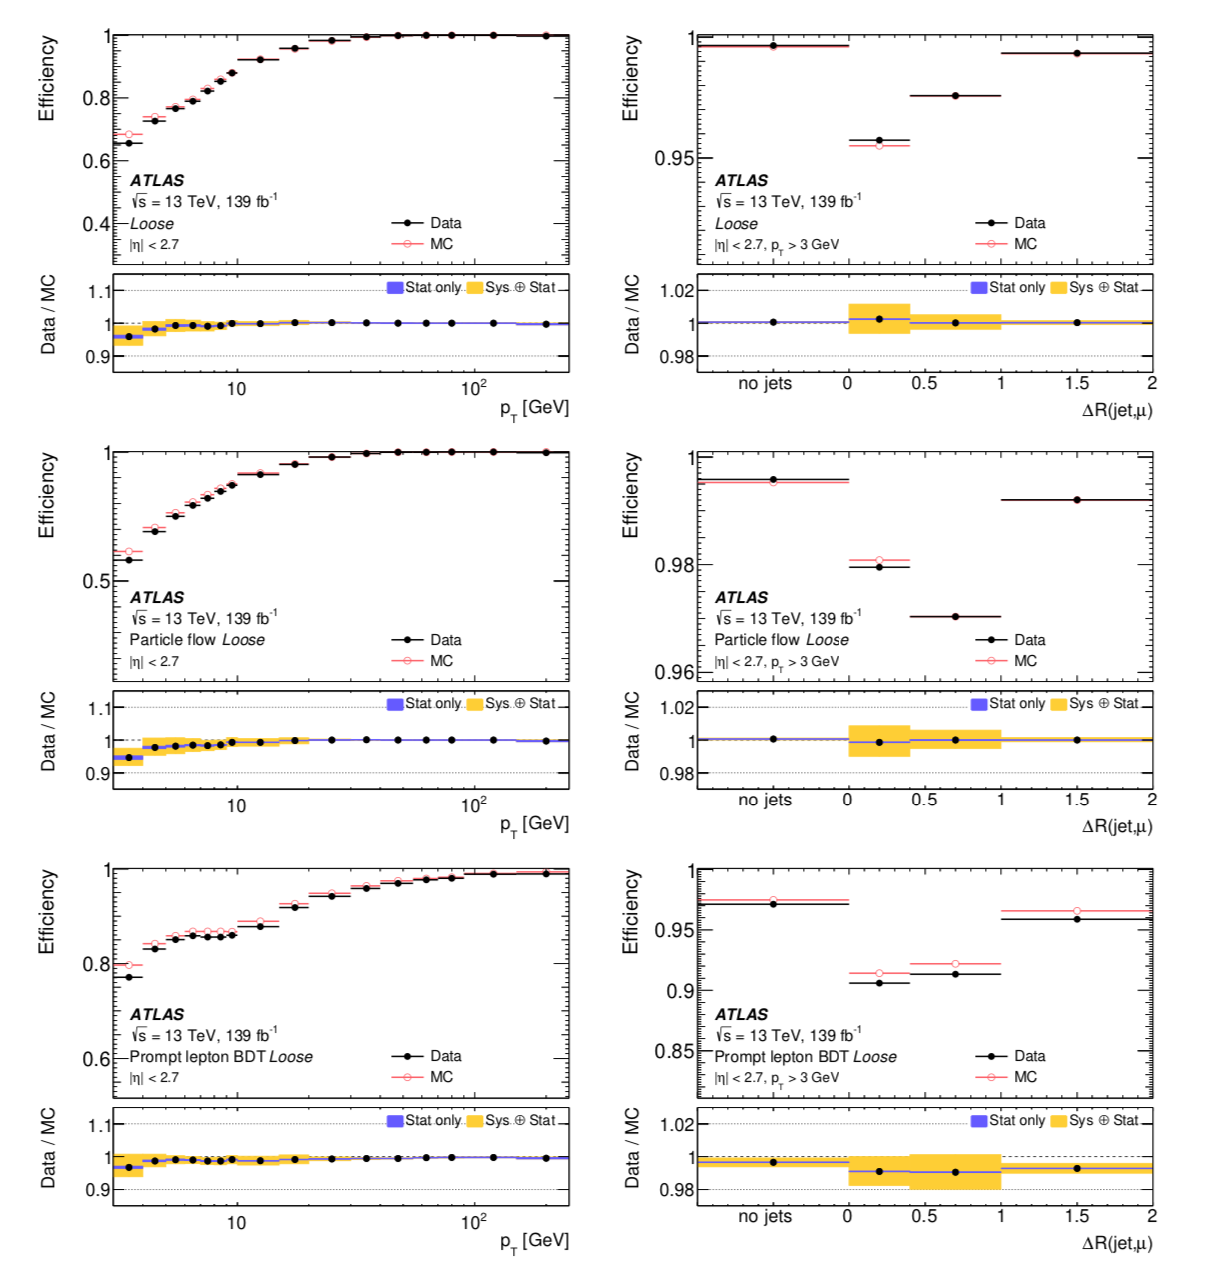
\includegraphics[width=0.75\textwidth]{figures/common_ana/IsolationEff1}
        %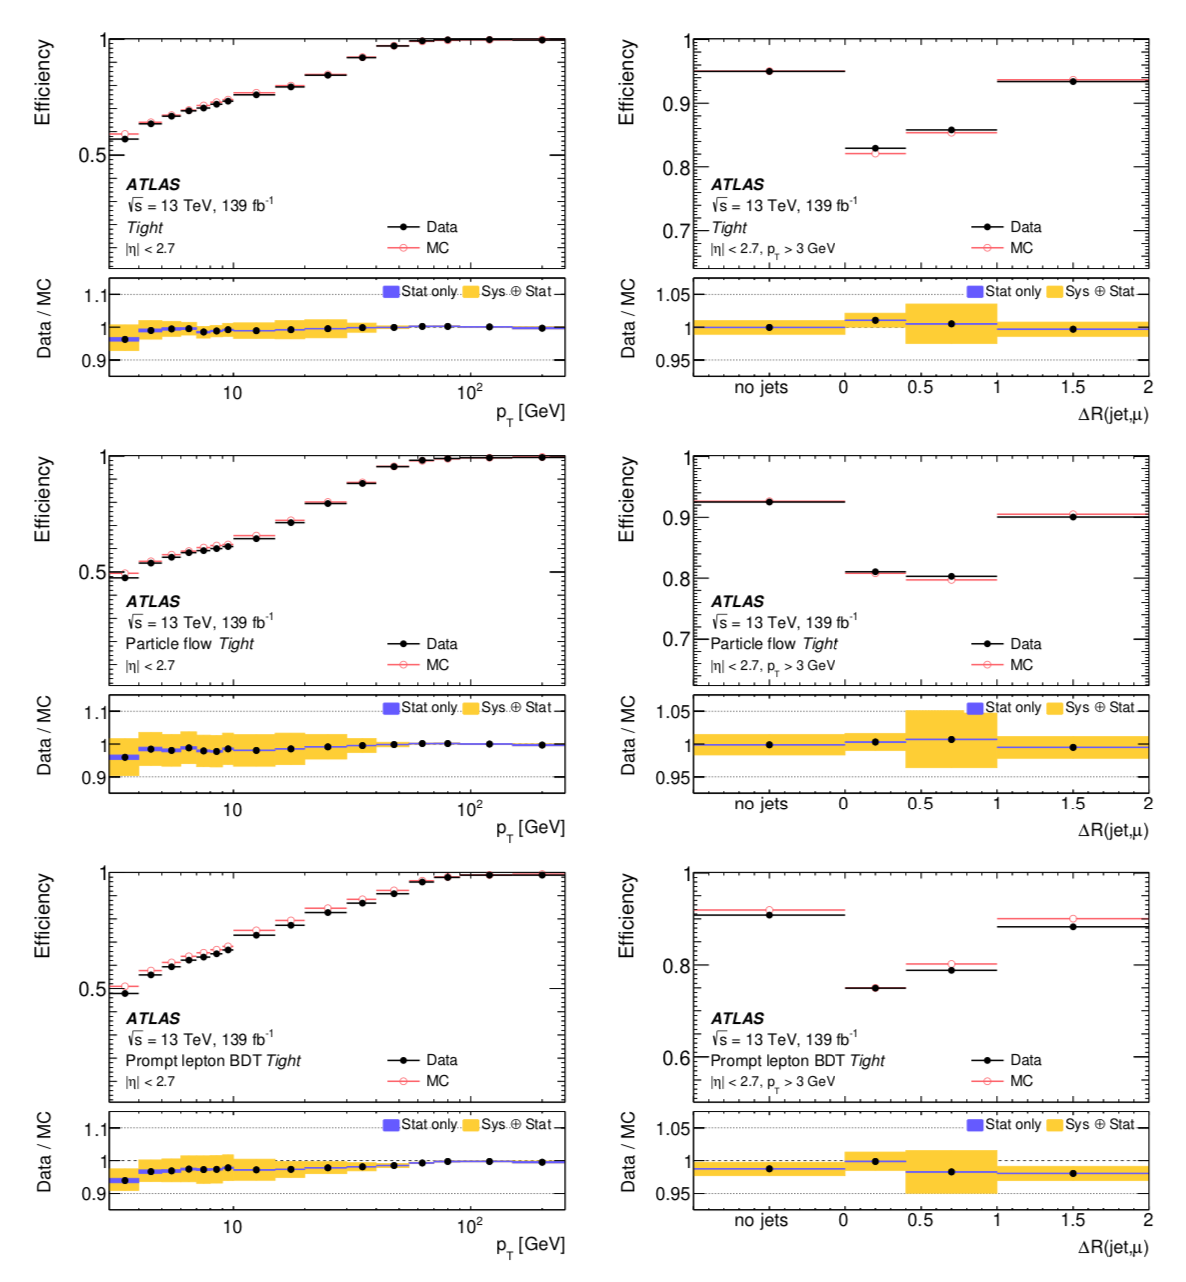
\includegraphics[width=0.75\textwidth]{figures/common_ana/IsolationEff2}
        \caption{
            This figure shows the isolation efficiency in different variable range in different working point\cite{Aad:2746302}.
        }
        \label{fig:isolationWP}
    \end{center}
\end{figure}


\subsection{Muon Calibration}
Given the difference between imperfect Monte Carlo generation and data, a calibration factor is derived from comparing the MC to data for some known physics process $J/\Psi$ to $\mu \mu$ and Z to $\mu \mu$. The calibration is done on the PT of the muon. 
The calibration is dependent on the detector angle, and the formula is summarized as below, where the constants are derived from the data and simulation of the samples.

%In data there is always margin for calibration error, and monte carlo is also not necessarily accurately describing the experimental environment. To match data result to the actual physics process that happened, transverse momentum correction done on both the MS tracks muons and the ID track on the MC result as follows: 

\begin{equation}

\[ P_{T}^{Cor,Det} = \frac{P^{MC, Det}_{T} + \sum_{n=0}^{1} S_{n}^{Det}{\eta, \phi}(P_{T}^{MC, Det})^n}{1+\sum_{m=0}^{2}\delta r_{m}^{Det}(\eta, \phi)(P_{T}^{MC, Det})^(m-1) g_{m}} \]
\label{eq:muoncalib}
\end{equation}


where $P_{T}^{MC, Det}$ is the uncorrected transverse momentum, $g_m$ is a unit Gausssian distribution, $\delta r^{Det}_{m}(\eta, \phi)$ and $s_{n}^{Det}(\eta, \phi)$ are the momentum resolution smearing and scale correction resolution. 

The correction is then applied to the combined muon in the following way:

\begin{equation}
\[ P_{T}^{Cor, CB} = f *P_{T}^{Cor, ID}+ (1-f) \cdot p_{T}^{Cor, MS}\]
\label{eq:muoncalibfactor}
\end{equation}

The weight f in the above is obtained from MC simulation. 



%\begin{equation}
%\[\delta R = min( \frac{10}/P_{T}[GeV] , \delta R_{max} )\]
%\end{equation}



%For better discrimination effciency, in Run II, ATLAS has moved away from an iterative based method and moved towards a image algorithm for primary vertex finding. A brief description is as the
%following:  
%
%1. A three-dimensional binned box is first defined, the x and y dimension is 4 mm long and the z dimension is 400 mm, a 3-d histogram is made for this 3d box as input data. 
%
%2. Helical tracks are back-projected back to this histogram using a voxel ray-tracking algorithm. All the histogram in each bin crossed by a track is incremented by the path length of the linearized rack in that bin. an example back projected in shown 
%% Whats a vortex ray-tracing algorithm? 
%
%3. This projection is Fourier transformed into frequency sapce.
%
%4. A filter composed of both the angular accpetance of the ATLAS tracking detector in the fourier inverse of the angular acceptance and a four-term Blackman-Harris window filter is used to lessen the effect of high frequency variation is used to multiplied by the projection in the above step. 
%
%5. The filtered image is then transformed back to position space in x, y and z.  
%
%5. The resulting imag is passed to a clustering algorithm where the seeds are identified from the peaks. 

\section{Jets}
Jets originate from either quarks or gluons form the p-p collision interaction vertices. Quarks and gluons follows rules from strong physics, they shower and scatter through the hadronization process, and therefore need to go through specific reconstruction steps to be reclustered back into a physical meaningful object for analysis. 

\subsection{Jet Physics}
Parton-parton scattering function in the LHC. 
Hadronization/ infrared and collinear safety

\subsection{Clustering}
The first step of reconstructing jet come first from a clustering of the calorimeter cells hits from the LAr and the tile calorimeters. First, seed-cells with a high signal-to-noise ratio is picked out to avoid pile-up. Then neighboring cells that satisfy  is chosen to add to the original seed cell. They form a proto-cluster. Proton clusters are merged if they satisfy merging requirements. The result of the clustering process is a collection of jet topo-clusters. 

\subsection{Jet finding}
There are a few main jet finding algorithms on ATLAS, which includes the $K_{T}$ algorithm, the Cambridge-A algorithm, and the anti-KT algorithm. 
\subsection{Calibration}
\subsection{Jet Origin Correction}


